\documentclass[a4paper, 11pt]{article}
\usepackage[utf8]{inputenc}
\usepackage[italian]{babel}
\usepackage{courier}
\usepackage{upgreek}

\usepackage[width=160mm, top=25mm, bottom=25mm]{geometry}

\usepackage{graphicx}
\usepackage{subfig}

\usepackage{amsmath}
\usepackage{bm}

% impostazioni per tabelle e grafici
\captionsetup{tableposition=bottom,figureposition=bottom,font=small} % impostazioni didascalie, vedi arte Latex di Pantieri
\captionsetup{format=hang,labelfont={sf,bf}} % NON OBBLIGATORIO -> VEDI SE TI PIACCIONO LE DIDASCALIE E IN CASO ELIMINA

\title{\textbf{Misura della caratteristica di uscita di un transistor BJT P-N-P in configurazione a emettitore comune}}
\author{Giada Martini \\ Lorenzo Calandra Buonaura}
\date{Turno 3 - 17 Novembre 2022}

\begin{document}

\maketitle

\section{Scopo della prova}
Lo scopo della prova è lo studio della caratteristica di uscita dal transistor BJT in configurazione a emettitore comune per valori fissati di corrente di base $I_B = -200 \mu A $ e $I_B = -100 \mu A$. 
%sinceramente non so cosa scrivere :)

\section{Schema del circuito}
\begin{figure}[!ht]
  \centering
  \begin{minipage}[b]{0.51\textwidth}
    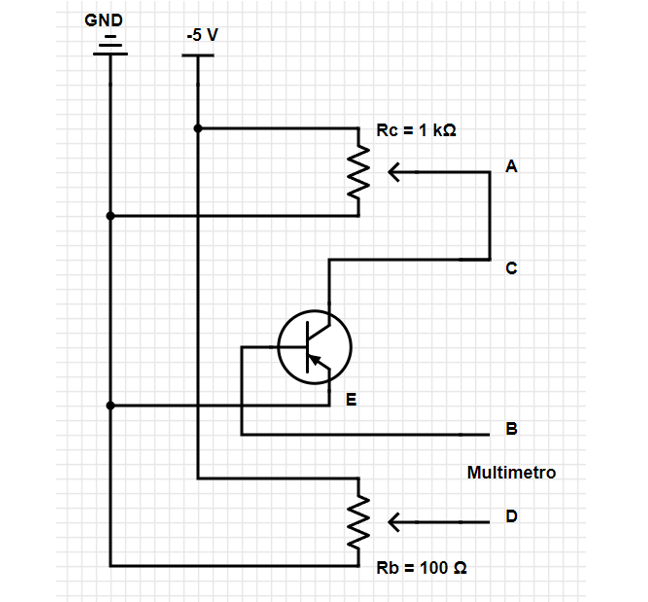
\includegraphics[width=76mm]{Schema circuito 1.png}
    \caption{\textit{Circuito utilizzato per settare la corrente \\ di base $I_B$ del transistor.}}
    \label{fig:Circuito per corrente di base}
  \end{minipage}
  \hfill
  \begin{minipage}[b]{0.48\textwidth}
    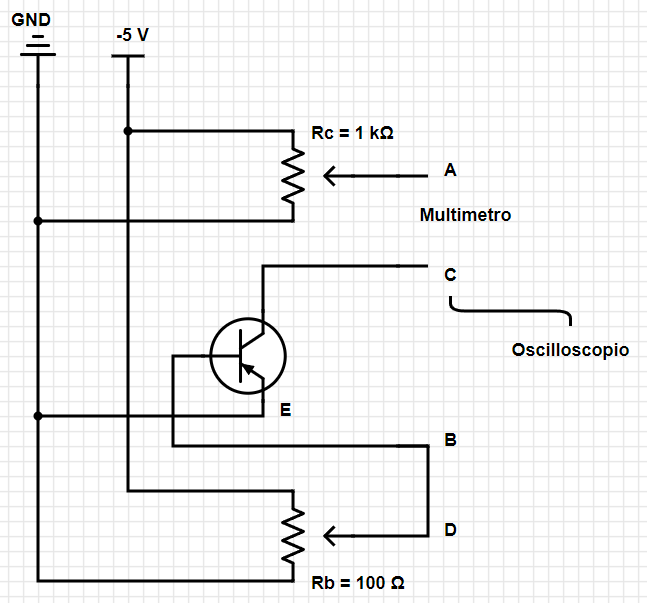
\includegraphics[width=76mm]{Schema circuito 2.png}
    \caption{\textit{Circuito utilizzato per la misura della caratteristica del transistor.}}
    \label{fig:Circuito utilizzato per la prova}
  \end{minipage}
\end{figure}

In Fig.\ref{fig:Circuito per corrente di base} si può vedere il circuito utilizzato per settare la corrente di base del transistor, prima a $I_B = -200 \mu A $ e poi $I_B = -100 \mu A$; in questo modo è stato possibile infatti impostare la corrente precisa, cortocircuitando i punti A e C del circuito e utilizzando il multimetro digitale collegato fra i punti B e D. In Fig. \ref{fig:Circuito utilizzato per la prova}, invece, si può vedere il circuito effettivamente utilizzato per raccogliere i dati durante l'esperienza; è stato cortocircuitato il collegamento fra B e D in modo da non modificare più la corrente di base e si è invece posizionato il multimetro fra A e C per misurare la corrente in uscita dal transistor. Inoltre al punto C è stato collegato anche l'oscilloscopio per le misure di tensione (ovviamente l'altro capo dell'oscilloscopio è collegato al GND).






\section{Strumenti e materiali utilizzati}
Per l'esperienza sono stati utilizzati i seguenti strumenti e materiali:
\begin{itemize}
    \item Alimentatore di bassa tensione, per fornire il valore del ground di riferimento e la differenza di potenziale di -5V.
    \item Multimetro digitale, per misurare i valori della corrente.
    \item Oscilloscopio, per misurare i valori di tensione.
    \item Potenziometro da 100 k$\Omega$ sulla base, fissato con una resistenza $R_B = 50 k\Omega$ e un potenziometro da $R_C = 1 k\Omega$ sulla corrente.
    \item Transistor BJT: 2N3906(BU) Silicio P-N-P in configurazione emettitore comune.
\end{itemize}


\section{Analisi dati}

\subsection{Caratteristica I-V del transistor BJT}
\begin{table}[!htb]
    \centering
    \begin{tabular}{|c|c|c|c|c|c|}
        \hline
        \bm{$V_{oscill.} (V)$} & \bm{$\sigma_{oscill.} (V)$} &         \bm{$I_{mult.} (mA)$} & \bm{$\sigma_{mult.} (mA)$} & \textbf{\textit{
        V/Div}} & \bm{$Range (mA)$} \\
        \hline
        4.00 & 0.52	& 36.42 & 0.57 & 1 & 32.00 \\ 
        \hline
        3.80 & 0.15 & 36.50 & 0.57 & 1 & 32.00 \\
        \hline
        3.60 & 0.15	& 36.60 & 0.57 & 1 & 32.00 \\
        \hline
        3.40 & 0.14 & 36.37 & 0.57 & 1 & 32.00 \\
        \hline
        3.20 & 0.14 & 36.24 & 0.56 & 1 & 32.00 \\
        \hline
        3.00 & 0.13 & 36.07 & 0.56 & 1 & 32.00 \\
        \hline
        2.80 & 0.13 & 35.79 & 0.56 & 1 & 32.00 \\
        \hline
        2.60 & 0.09 & 35.58 & 0.55 & 0.5 & 32.00 \\
        \hline
        2.40 & 0.09 & 35.29 & 0.55 & 0.5 & 32.00 \\
        \hline 
        2.20 & 0.08 & 34.91 & 0.54 & 0.5 & 32.00 \\
        \hline
        2.00 & 0.08 & 34.50 & 0.54 & 0.5 & 32.00 \\
        \hline
        1.80 & 0.07 & 34.12 & 0.53 & 0.5 & 32.00 \\
        \hline
        1.60 & 0.07 & 33.61 & 0.52 & 0.5 & 32.00 \\
        \hline
        1.40 & 0.07 & 32.92 & 0.51 & 0.5 & 32.00 \\
        \hline        
        1.20 & 0.06 & 32.34 & 0.51 & 0.5 & 32.00 \\
        \hline
        1.00 & 0.06 & 31.60 & 0.49 & 0.5 & 32.00 \\
        \hline
        0.96 & 0.04 & 31.45 & 0.49 & 0.2 & 32.00 \\
        \hline 
        0.88 & 0.03 & 31.10 & 0.49 & 0.2 & 32.00 \\
        \hline
        0.80 & 0.03 & 30.72 & 0.48 & 0.2 & 32.00 \\
        \hline 
        0.68 & 0.03 & 29.95 & 0.47 & 0.2 & 32.00 \\
        \hline 
        0.60 & 0.03 & 29.07 & 0.46 & 0.2 & 32.00 \\
        \hline 
        0.48 & 0.02 & 27.29 & 0.43 & 0.2 & 32.00 \\
        \hline
        0.40 & 0.02 & 25.62 & 0.40 & 0.2 & 32.00 \\
        \hline 
        0.32 & 0.01 & 24.62 & 0.39 & 0.1 & 32.00 \\
        \hline 
        0.30 & 0.01 & 23.42 & 0.37 & 0.1 & 32.00 \\
        \hline 
        0.24 & 0.01 & 20.48 & 0.33 & 0.1 & 32.00 \\
        \hline 
        0.20 & 0.01 & 17.27 & 0.28 & 0.1 & 32.00 \\
        \hline 
        0.15 & 0.01 & 12.24 & 0.20 & 0.05 & 32.00 \\
        \hline 
        0.12 & 0.01 & 7.65 & 0.13 &	0.05 & 32.00 \\
        \hline 
        0.10 & 0.01 & 4.87 & 0.09 &	0.05 & 32.00 \\
        \hline 
        0.05 & 0.01 & 0.74 & 0.03 &	0.05 & 32.00 \\
        \hline 
    \end{tabular} 
    \caption{Valori di tensione e corrente misurati per corrente $I_B = -0.2 mA$.}
    \label{tab:-0.2 mA}
\end{table}


\begin{table}[!htb]
    \centering
    \begin{tabular}{|c|c|c|c|c|c|}
        \hline
        \bm{$V_{oscill.} (V)$} & \bm{$\sigma_{oscill.} (V)$} &         \bm{$I_{mult.} (mA)$} & \bm{$\sigma_{mult.} (mA)$} & \textbf{\textit{V/Div}} & \bm{$Range (mA)$} \\
        \hline
        4.00 & 0.52 & 19.62 & 0.31 & 1.00 & 32.00 \\
        \hline 
        3.80 & 0.15 & 19.64 & 0.31 & 1.00 & 32.00 \\
        \hline 
        3.60 & 0.15 & 19.63 & 0.31 & 1.00 & 32.00 \\
        \hline 
        3.40 & 0.14 & 19.55 & 0.31 & 1.00 & 32.00 \\
        \hline
        3.20 & 0.14 & 19.51 & 0.31 & 1.00 & 32.00 \\
        \hline 
        3.00 & 0.13 & 19.46 & 0.31 & 1.00 & 32.00 \\
        \hline 
        2.80 & 0.13 & 19.28 & 0.31 & 1.00 & 32.00 \\
        \hline 
        2.60 & 0.09 & 19.25 & 0.31 & 0.50 & 32.00 \\
        \hline 
        2.40 & 0.09 & 19.13 & 0.31 & 0.50 & 32.00 \\
        \hline 
        2.20 & 0.08 & 19.07 & 0.31 & 0.50 & 32.00 \\
        \hline 
        2.00 & 0.08 & 18.86 & 0.30 & 0.50 & 32.00 \\
        \hline 
        1.80 & 0.07 & 18.65 & 0.30 & 0.50 & 32.00 \\
        \hline 
        1.60 & 0.07 & 18.45 & 0.30 & 0.50 & 32.00 \\
        \hline 
        1.40 & 0.07 & 18.26 & 0.29 & 0.50 & 32.00 \\
        \hline 
        1.20 & 0.06 & 18.05 & 0.29 & 0.50 & 32.00 \\
        \hline 
        1.00 & 0.06 & 17.80 & 0.29 & 0.50 & 32.00 \\
        \hline 
        0.96 & 0.04 & 17.68 & 0.29 & 0.20 & 32.00 \\
        \hline 
        0.88 & 0.03 & 17.54 & 0.28 & 0.20 & 32.00 \\
        \hline 
        0.80 & 0.03 & 17.42 & 0.28 & 0.20 & 32.00 \\
        \hline 
        0.68 & 0.03 & 17.22 & 0.28 & 0.20 & 32.00 \\
        \hline 
        0.60 & 0.03 & 17.07 & 0.28 & 0.20 & 32.00 \\
        \hline 
        0.48 & 0.02 & 16.72 & 0.27 & 0.20 & 32.00 \\
        \hline 
        0.40 & 0.02 & 16.29 & 0.26 & 0.20 & 32.00 \\
        \hline 
        0.32 & 0.01 & 15.59 & 0.25 & 0.10 & 32.00 \\
        \hline 
        0.30 & 0.01 & 15.24 & 0.25 & 0.10 & 32.00 \\
        \hline 
        0.24 & 0.01 & 13.83 & 0.23 & 0.10 & 32.00 \\
        \hline 
        0.20 & 0.01 & 11.78 & 0.20 & 0.10 & 32.00 \\
        \hline 
        0.15 & 0.01 & 8.32 & 0.14 & 0.05 & 32.00 \\
        \hline 
        0.12 & 0.01 & 4.94 & 0.09 &	0.05 & 32.00 \\
        \hline 
        0.10 & 0.01 & 3.01 & 0.07 &	0.05 & 32.00 \\
        \hline 
        0.05 & 0.01 & 0.44 & 0.03 &	0.05 & 32.00 \\
        \hline 
    \end{tabular} 
    \caption{Valori di tensione e corrente misurati per corrente $I_B = -0.1 mA$.}
    \label{tab:-0.1 mA}
\end{table}


%DOBBIAMO GUAARDARE IL RANGE E NON RICORDO SE VOLT O MVOLT 
\section{Risultati finali e conclusioni}

\section{Appendice}

\end{document}
